\subsubsection{The SolKz Stokes benchmark}
\label{sec:benchmark-solkz}

The SolKz benchmark is another variation on the same theme as the SolCx
benchmark above: it solves a Stokes problem with a spatially variable
viscosity, but this time the viscosity is not a discontinuous function. Instead,
it grows exponentially with the vertical coordinate so that its overall
variation is again $10^6$. The forcing is again chosen by imposing a spatially
variable density variation. For details, refer again to \cite{DMGT11}.

The following input file, only a small variation of the one in the previous
section, solves the benchmark (see \url{benchmarks/solkz/}):

\lstinputlisting[language=prmfile]{cookbooks/benchmarks/solkz/doc/solkz.prm.out}

The output when running \aspect{} on this parameter file looks similar to the
one shown for the SolCx case. The solution when computed with one more level
of global refinement is visualized in Fig.~\ref{fig:solkz}. The velocity solution
computed with three more levels of global refinement and plotted over the viscosity
field is shown in Fig.~\ref{fig:solkz2}.

\begin{figure}
  \begin{center}
    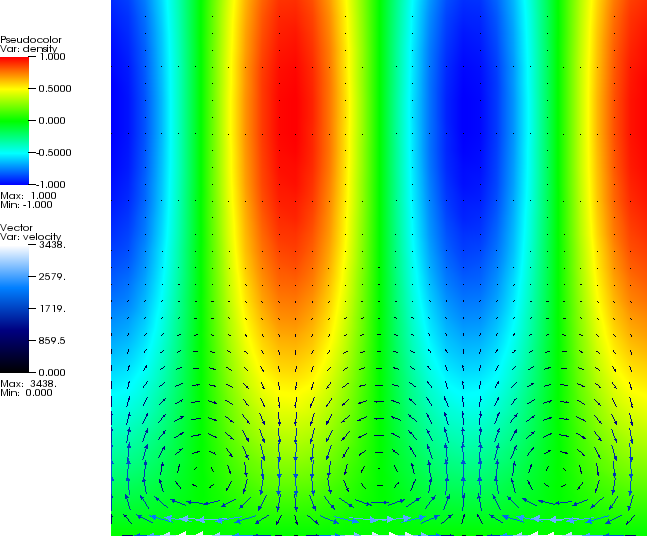
\includegraphics[width=0.45\textwidth]{cookbooks/benchmarks/solkz/doc/solkz-solution.png}
    \hfill
    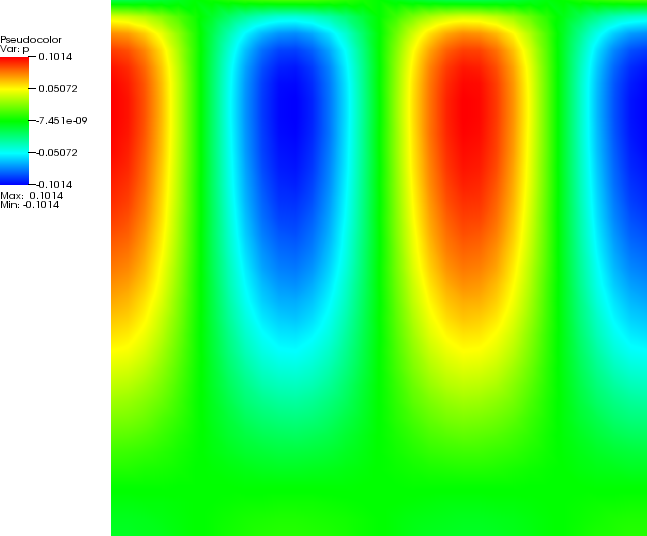
\includegraphics[width=0.45\textwidth]{cookbooks/benchmarks/solkz/doc/solkz-solution-pressure.png}
    \caption{\it SolKz Stokes benchmark. Left: The density perturbation field
    overlaid with velocity vectors. The viscosity grows exponentially
      in the vertical direction, leading to small velocities at the top
      despite the large density variations. Right: The pressure.}
    \label{fig:solkz}
  \end{center}
\end{figure}

\begin{figure}
  \begin{center}
    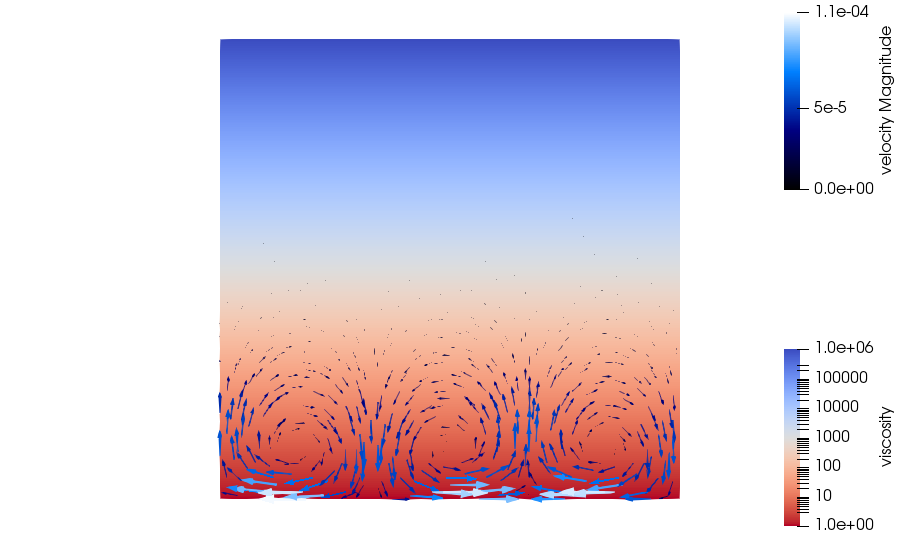
\includegraphics[width=0.7\textwidth]{cookbooks/benchmarks/solkz/doc/solkz-solution-viscosity.png}
    \caption{\it SolKz Stokes benchmark. Another view of the velocity vectors, this time plotted over the viscosity field.}
    \label{fig:solkz2}
  \end{center}
\end{figure}
